%!TEX program = lualatex

%------------------------------------------------
% PARTE 1 - IMPOSTAZIONI GENERALI DEL DOCUMENTO
% In questa parte ci sono i pacchetti LaTeX
% utilizzati, il carattere e la dimensione
% del testo. Vi è anche la definizione
% linguaggio JSON quando si scrive testo che
% deve essere formattato in questo linguaggio
%------------------------------------------------


\documentclass[10pt, titlepage]{report}


% Pacchetti
\usepackage{graphicx}
\usepackage{float}
\usepackage{listings}
\usepackage{xcolor}
\usepackage[italian]{babel}
\usepackage{subfig}
\usepackage{tabularx}
\usepackage[T1]{fontenc}
\usepackage{afterpage}
\usepackage{multirow}
\usepackage{makecell}
\usepackage{enumerate}


%Impostazioni testo
\usepackage{geometry}
 \geometry{
 	a4paper,
 	left=3cm,
 	right=3cm,
 	top=3cm,
 	bottom=3cm
 }
\usepackage{fontspec}
\setmainfont{Arial}
\linespread{1.5}


%Impostazioni
\newcommand*{\chapterpath}{capitoli}
\graphicspath{ {img/} }

\colorlet{punct}{red!60!black}
\definecolor{background}{HTML}{EEEEEE}
\definecolor{delim}{RGB}{20,105,176}
\colorlet{numb}{magenta!60!black}

% Definizione JSON
\lstdefinelanguage{json}{
	basicstyle=\normalfont\ttfamily,
	numberstyle=\scriptsize,
	stepnumber=1,
	numbersep=4pt,
	showstringspaces=false,
	breaklines=true
}



%--------------------------------------------------
% PARTE 2 - IMPOSTAZIONI SPECIFICHE DEL DOCUMENTO
% In questa parte ci sono il titolo,
% il frontespizio, i capitoli e la bibliografia
%--------------------------------------------------

%Titolo
\title{Titolo della tesi}
\author{Nome e cognome}
\date{01/01/2000}

%Documento
\begin{document}

% Frontespizio
\begin{titlepage}
    \begin{center}
        
\includegraphics[width=0.4\textwidth]{logo_uniba}\\
        \vspace{1cm}
        % Dipartimento
        {\large Dipartimento di Inserire il dipartimento}\\
        \vspace{1cm}
        % Corso di laurea
        {\large Corso di laurea in Inserire il corso di laurea}\\
        \hrulefill \\
        \vspace{2cm}
        {\large \textbf{TESI DI LAUREA IN}}\\
        \vspace{0.5cm}
        % Materia
        {\large Materia delle tesi}\\
        \vspace{2cm}
        % Titolo
        {\LARGE\textbf{Inserire qui il titolo della tesi}}\\
        \vspace{2cm}

        \vfill
        
        \begin{tabularx}{\textwidth}{@{}lX}
          & \\
          & {\large Relatore:} \\
          % Relatore
          & {\large \textbf{Prof. Nome Cognome}}
        \end{tabularx}

        \begin{tabularx}{\textwidth}{@{}lX}
            & \\
            & {\large Corelatore:} \\
            % Corelatore
            & {\large \textbf{Prof. Nome Cognome}}
          \end{tabularx}

        \begin{tabularx}{\textwidth}{Xr@{}}
          & \\
          & {\large Laureando:} \\
          % Laureando
          & {\large \textbf{Nome Cognome}}
        \end{tabularx}

        \vspace{1cm}
        \hrulefill \\
        \vspace{1cm}
        % Anno accademico in cui si è iscritti
        {\large Anno Accademico \textbf{2021-2022}}
    \end{center}
\end{titlepage}

% Abstract
\selectlanguage{english}
\renewcommand{\abstractname}{Abstract}  % Per avere il titolo "Abstract" invece di "Sommario"
\begin{abstract}
    Inserire qui l'abstract della tesi.\\
    Lorem ipsum dolor sit amet, consectetur adipiscing elit, sed do eiusmod tempor incididunt ut labore et dolore magna aliqua. Ut enim ad minim veniam, quis nostrud exercitation ullamco laboris nisi ut aliquip ex ea commodo consequat. Duis aute irure dolor in reprehenderit in voluptate velit esse cillum dolore eu fugiat nulla pariatur. Excepteur sint occaecat cupidatat non proident, sunt in culpa qui officia deserunt mollit anim id est laborum.
\end{abstract}
\selectlanguage{italian}

%Indice
\tableofcontents

% Capitoli
\chapter{Sezioni e paragrafi}
Questo è il secondo capitolo. Qui verranno inserite e spiegate le varie sezioni, sottosezioni e paragrafi.

\section{Prima sezione}
Questa è la prima sezione del capitolo.

\subsection{Sezione interna alla prima sezione}
Con questo comando inserisco una sezione interna al precedente \textit{section}.

\subsubsection{Sezione interna alla sezione interna}
Terzo livello di sezione. Questa non è numerata.

\section{Seconda sezione}
Digitando il comando \textit{section}, viene inserita subito una nuova sezione. Spostando la sezione in qualsiasi punto del documento, i numeri verranno reinseriti automaticamente.

\paragraph{} Esempio di paragrafo senza titolo. Lorem ipsum dolor sit amet, consectetur adipiscing elit, sed do eiusmod tempor incididunt ut labore et dolore magna aliqua. Ut enim ad minim veniam, quis nostrud exercitation ullamco laboris nisi ut aliquip ex ea commodo consequat. Duis aute irure dolor in reprehenderit in voluptate velit esse cillum dolore eu fugiat nulla pariatur. Excepteur sint occaecat cupidatat non proident, sunt in culpa qui officia deserunt mollit anim id est laborum.

\paragraph{Paragrafo con titolo.} Esempio di paragrafo con il titolo. Lorem ipsum dolor sit amet, consectetur adipiscing elit, sed do eiusmod tempor incididunt ut labore et dolore magna aliqua. Ut enim ad minim veniam, quis nostrud exercitation ullamco laboris nisi ut aliquip ex ea commodo consequat. Duis aute irure dolor in reprehenderit in voluptate velit esse cillum dolore eu fugiat nulla pariatur. Excepteur sint occaecat cupidatat non proident, sunt in culpa qui officia deserunt mollit anim id est laborum.
\chapter{Immagini, tabelle, codice, liste}
In questo capitolo verranno spiegati tutti i comandi per inserire codice, tabelle di varie dimensioni, elenchi, immagini ecc.


\section{Liste}
Le liste possono essere sia numerate che puntate. La prima lista mostra come si scrivono alcuni caratteri e come si definisce lo stile di scrittura:
\begin{itemize}
    \item si può scrivere in \textbf{grassetto};
    \item si può scrivere in \textit{corsivo};
    \item si può inserire il carattere \& per la e commerciale;
    \item si può inserire il carattere \_ per l'underscore;
\end{itemize}

Ci sono anche gli elenchi numerati classici:
\begin{enumerate}
    \item primo elemento;
    \item secondo elemento;
    \item terzo elemento.
\end{enumerate}

Ma anche gli elenchi in numeri romani:
\begin{enumerate}[I]    % sostituendo 'I' con 'i' l'elenco sarà con i numeri romani minuscoli.
    \item primo elemento in romano;
    \item secondo elemento in romano;
    \item terzo elemento in romano;
    \item quarto elemento in romano.
\end{enumerate}


\section{Immagini}
Durante la produzione del testo può essere utile avere un'immagine o una serie di immagini.

\begin{figure}[H]
	\centering
	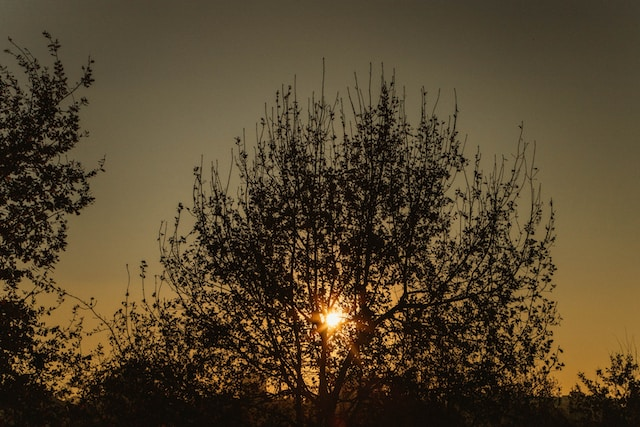
\includegraphics[scale=0.4]{image1} % Non è necessario specificare l'estensione. L'immagine viene pescata automaticamente dalla cartella 'img' per cui non è necessario scrivere il percorso completo
	\caption{Immagine singola centrata e scalata \cite{unsplashImage1}}
	\label{capitolo2:image1}
\end{figure}

È possibile fare riferimento alle immagini attraverso la sua label (figura \ref{capitolo2:image1}).\\   % Con questo \\ si va a capo
In altri casi è necessario avere più immagini affiancate.

\begin{figure}[H]
    \centering
    \subfloat[Immagine 1 \cite{unsplashImage2a}]{
\includegraphics[scale=0.2]{image2a}}
    \hfill
    \subfloat[Immagine 2 \cite{unsplashImage2b}]{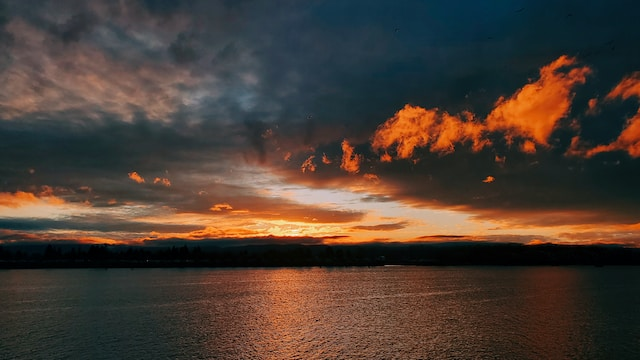
\includegraphics[scale=0.2]{image2b}}
    \hfill
    \subfloat[Immagine 3 \cite{unsplashImage2c}]{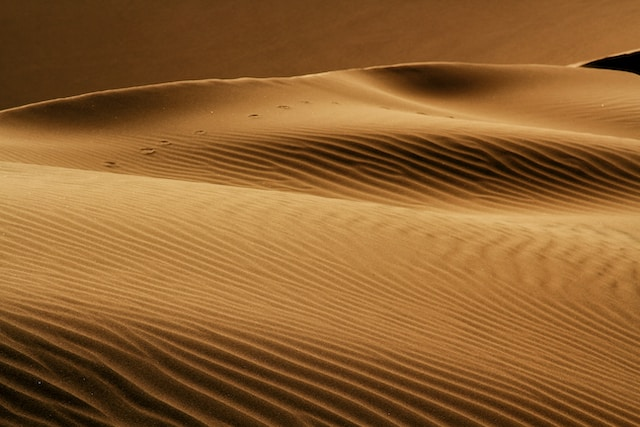
\includegraphics[scale=0.2]{image2c}}
    \hfill
    \caption{Immagini affiancate al centro}
    \label{capitolo2:immaginiAffiancate}
\end{figure}


\section{Tabelle}
Le tabelle possono avere varie dimensioni. Qui ne verranno mostrate 2: una con una dimensione normale e una con una dimensione maggiore per mostrare come si adattano alla pagina.
\begin{table}[h!]
    \centering
    \begin{tabular}{|c|c|c|}
        \hline
        \textbf{Colonna 1} & \textbf{Colonna 2} & \textbf{Colonna 3} \\
        \hline
        Dato 1 & 10 & Testo A \\
        \hline
        Dato 2 & 5.6 & Testo B \\
        \hline
        Dato 3 & 7.2 & Testo C \\
        \hline
    \end{tabular}
    \caption{Tabella piccola}
	\label{capitolo2:tabellaPiccola}
\end{table}

Quella che segue è una tabella più grande e adattata alla pagina, in modo da essere stampabile.

\begin{table}[h!]
	\centering
    \small
	\begin{tabular}{| c | c | c | c | c | c | c || c |}
		\hline \textbf{Colonna 1} & \textbf{Colonna 2} & \textbf{Colonna 3} & \textbf{Colonna 4} & \textbf{Colonna 5} & \textbf{Colonna 6} & \textbf{Colonna 7} & \textbf{Colonna 8} \\ [0.5ex]
		\hline\hline
		Dato 1 & 12 & \makecell{Testo che per \\ questioni di \\ spazio va a capo} & 3.4 & 5 & Testo X & 0.7 & \textbf{34.1} \\
		\hline
		Dato 2 & 8.9 & Testo B & 1.2 & 2 & Testo Y & 0.3 & \textbf{12.4} \\
		\hline
		Dato 3 & 15 & Testo C & 4.8 & 3 & Testo Z & 0.9 & \textbf{23.7} \\
		\hline
        Dato 4 & 6.5 & Testo D & 2.1 & 1 & Testo W & 0.5 & \textbf{10.6} \\
        \hline
        Dato 5 & 9.2 & Testo E & 5.3 & 4 & Testo V & 0.8 & \textbf{30.5} \\
        \hline
        Dato 6 & 14 & Testo F & 3.2 & 2 & Testo U & 0.4 & \textbf{21.6} \\
        \hline
        Dato 7 & 7.8 & Testo G & 1.5 & 3 & Testo T & 0.6 & \textbf{13.9} \\
        \hline
        Dato 8 & 10.1 & Testo H & 4.5 & 4 & Testo S & 0.7 & \textbf{30.3} \\
        \hline
        Dato 9 & 5.3 & Testo I & 2.8 & 1 & Testo R & 0.2 & \textbf{9.1} \\
        \hline
        Dato 10 & 11.5 & Testo J & 3.7 & 2 & Testo Q & 0.9 & \textbf{32.8} \\
        \hline
	\end{tabular}
	\caption{Tabella grande}
	\label{capitolo2:tabellaGrande}
\end{table}


\section{Codice}
Qui verranno mostrati due esempi di codice sia in Python che in JSON.

\begin{lstlisting}[language=json, basicstyle=\small, caption={Esempio JSON}, label=capitolo2:code:json]
{
  "nome": "John Doe",
  "eta": 30,
  "professione": "Ingegnere",
  "indirizzo": {"via": "Via delle Rose, 123", "citta": "Città del Sole", "cap": "12345"},
  "interessi": ["musica", "viaggi", "sport"],
  "esperienze_lavorative": [{"azienda": "ABC Inc.", "posizione": "Sviluppatore software", "periodo": "2010-2015"}, {"azienda": "XYZ Corp.", "posizione": "Project Manager", "periodo": "2015-2020"}],
  "lingue": {"inglese": "fluente", "italiano": "madrelingua", "spagnolo": "intermedio"},
  "referenze": null,
  "disponibile": true
}
\end{lstlisting}

Ecco un esempio del linguaggio Python.

\begin{lstlisting}[language=python, basicstyle=\small, caption={Esempio Python}, label=capitolo2:code:python]
def somma(a, b):
return a + b

numero1 = 5
numero2 = 7

risultato = somma(numero1, numero2)
print("La somma di", numero1, "e", numero2, "è:", risultato)

\end{lstlisting}


\section{Formule matematiche}
È possibile inserire formule matematiche durante il testo e ce ne sono di due tipi. La prima si inserisce all'interno del testo: $f(x) = \frac{x^2}{2}$, mentre il secondo si inserisce in una nuova riga.
\begin{equation}
    \sum_{i=0}^{\infty} \alpha\sin{x_i}
    \label{capitolo2:eq:esempioEquazione}
\end{equation}
Anche in questo caso, tramite la label, è possibile fare riferimento a questa formula in qualsiasi punto del documento, esattamente come per immagini, tabelle e codice.

\end{document}